\documentclass{book}

\usepackage{tikz}
\usetikzlibrary{positioning,arrows.meta,calc,decorations.pathreplacing}
%\usepackage[dvipsnames]{xcolor}

% relative positioning
%\usetikzlibrary{positioning}

% braces
%\usetikzlibrary{decorations.pathreplacing}

% autoencoder
%\usetikzlibrary{positioning,arrows.meta,calc,decorations.pathreplacing}

% actvation functions tikz
\usepackage{subfigure}
\usepackage{pgfplots}
\pgfplotsset{compat=1.16}
\usepackage[top=3cm,left=3cm,right=3cm,bottom=3cm,
%    showframe
]{geometry}
% Scriptsize axis style.
\pgfplotsset{every axis/.append style={tick label style={/pgf/number format/fixed},font=\scriptsize,ylabel near ticks,xlabel near ticks,grid=major}}

%\def\layersep{3em}
%\def\transferx{9em}
%\def\hiddenx{7em}
%\def\hiddenxn{12em}

\begin{document}

    % venn
    \begin{figure}[!htp]
        \centering
        \input{src/ai-ml-dl.tex}
        \caption{
            The relation between the field of Artificial Intelligence,
            Machine Learning, Deep Learning and Reinforcement Learning.
        }
        \label{fig:al-ml-dl}
    \end{figure}

    % perceptron
    \begin{figure}[!htp]
        \centering
        % MIT License
%
% Copyright (c) 2021 Geoffrey H. Garrett
%
% Permission is hereby granted, free of charge, to any person obtaining a copy
% of this software and associated documentation files (the "Software"), to deal
% in the Software without restriction, including without limitation the rights
% to use, copy, modify, merge, publish, distribute, sublicense, and/or sell
% copies of the Software, and to permit persons to whom the Software is
% furnished to do so, subject to the following conditions:
%
% The above copyright notice and this permission notice shall be included in all
% copies or substantial portions of the Software.
%
% THE SOFTWARE IS PROVIDED "AS IS", WITHOUT WARRANTY OF ANY KIND, EXPRESS OR
% IMPLIED, INCLUDING BUT NOT LIMITED TO THE WARRANTIES OF MERCHANTABILITY,
% FITNESS FOR A PARTICULAR PURPOSE AND NONINFRINGEMENT. IN NO EVENT SHALL THE
% AUTHORS OR COPYRIGHT HOLDERS BE LIABLE FOR ANY CLAIM, DAMAGES OR OTHER
% LIABILITY, WHETHER IN AN ACTION OF CONTRACT, TORT OR OTHERWISE, ARISING FROM,
% OUT OF OR IN CONNECTION WITH THE SOFTWARE OR THE USE OR OTHER DEALINGS IN THE
% SOFTWARE.

%%%%%%%%%%%%%%%%%%%%%%%%%%%%%%%%%%%%%%%%%%%%%%%%%%%%%%%%%%%%%%%%%%%%%%%%%%%%%%%
% ACKNOWLEDGEMENTS
%%%%%%%%%%%%%%%%%%%%%%%%%%%%%%%%%%%%%%%%%%%%%%%%%%%%%%%%%%%%%%%%%%%%%%%%%%%%%%%
% Design and implementation of this diagram was inspired and adapted from:
% https://tex.stackexchange.com/questions/104334/tikz-diagram-of-a-perceptron

%%%%%%%%%%%%%%%%%%%%%%%%%%%%%%%%%%%%%%%%%%%%%%%%%%%%%%%%%%%%%%%%%%%%%%%%%%%%%%%
% DEPENDENCIES
%%%%%%%%%%%%%%%%%%%%%%%%%%%%%%%%%%%%%%%%%%%%%%%%%%%%%%%%%%%%%%%%%%%%%%%%%%%%%%%
%\usepackage{tikz}
%\usetikzlibrary{decorations.pathreplacing}    % for TikZ braces
%\usetikzlibrary{positioning}                  % for TikZ relative positioning

%%%%%%%%%%%%%%%%%%%%%%%%%%%%%%%%%%%%%%%%%%%%%%%%%%%%%%%%%%%%%%%%%%%%%%%%%%%%%%%
% USER STYLING
%%%%%%%%%%%%%%%%%%%%%%%%%%%%%%%%%%%%%%%%%%%%%%%%%%%%%%%%%%%%%%%%%%%%%%%%%%%%%%%

% TikZ node design.
\tikzset{basic/.style={draw,text width=1em,text badly centered}}
\tikzset{input/.style={}}
\tikzset{output/.style={}}
\tikzset{weight/.style={basic,circle}}
\tikzset{hidden/.style={basic,circle}}
\tikzset{function/.style={basic,circle}}

% Labels and symbols.
\def\activationlabel{activation function}  % activation function label
\def\activationsymbol{$\phi$}              % activation function symbol
\def\transferlabel{transfer function}      % transfer function label
\def\transfersymbol{$\sum$}                % transfer function symbol
\def\outputsymbol{$y$}                     % output symbol
\def\inputsymbol{$x$}                      % input symbol
\def\inputvecsymbol{$\mathbf{x}$}          % input vector symbol
\def\weightslabel{weights}                 % input vector symbol
\def\biassymbol{$b$}                       % bias symbol

%%%%%%%%%%%%%%%%%%%%%%%%%%%%%%%%%%%%%%%%%%%%%%%%%%%%%%%%%%%%%%%%%%%%%%%%%%%%%%%
% TIKZ PICTURE
%%%%%%%%%%%%%%%%%%%%%%%%%%%%%%%%%%%%%%%%%%%%%%%%%%%%%%%%%%%%%%%%%%%%%%%%%%%%%%%
\begin{tikzpicture}
    \node[function] at ({\transferx}, -{int(2)})  (transfer) {\transfersymbol};
    \node[function, right=3em of transfer] (activation) {\activationsymbol};
    \node[below of=activation,font=\scriptsize,text width=3em] {\activationlabel};
    \node[below of=transfer,font=\scriptsize,text width=3em] {\transferlabel};
    \node[output, right=\layersep of activation] (output) {\outputsymbol};
    \path[draw,->] (transfer) -- (activation);
    \path[draw,->] (activation) -- (output);

    % Iterate through each row of units.
    \foreach \n [evaluate=\n as \p using {int(\n-1)}] in {0,1,2,3,4} {
        \ifnum \n=0
        \node[input] at (0, -\n) (X-\n) {$1$};
        \node[weight] at (\layersep, -\n) (W-\n) {$w_\n$};
        \else \ifnum \n=3
        \node[] at (0, -\n) (X-\n) {$\vdots$};
        \node[] at (\layersep, -\n) (W-\n) {$\vdots$};
        \else \ifnum \n=4
        \node[input] at (0, -\n) (X-\n) {$x_{d_{{in}}}$};
        \node[weight,label={[xshift=-0.0em]center:$w_{d_{{in}}}$}] at (\layersep, -\n) (W-\n) {\phantom{$w_{d_{{in}}}$}};
        \else
        \node[input] at (0, -\n) (X-\n) {$x_\n$};
        \node[weight] at (\layersep, -\n) (W-\n) {$w_\n$};
        \fi
        \fi
        \fi

        % Arrow from input to weight.
        \ifnum \n=3
        \else
        \path[draw,->] (X-\n) -- (W-\n);
                    \path[draw,->] (W-\n) -- (transfer);
        \fi

    }

    % Brace for bias.
    \node[left=1em of X-0] (bias-brace) {};
    \node[above=1em of bias-brace] (bias-brace-up) {};
    \node[below=1em of bias-brace] (bias-brace-down) {};
    \draw[decorate,decoration = {brace}] (bias-brace-down) --  (bias-brace-up);
    \node[left of=bias-brace,font=\scriptsize] {bias, \biassymbol};

    % Brace for input.
    \node[below=10em of bias-brace-down] (input-brace-down) {};
    \node[below=5em of bias-brace-down] (input-brace) {};
    \draw[decorate,decoration = {brace}] (input-brace-down) --  (bias-brace-down);
    \node[left of=input-brace,font=\scriptsize] {inputs, \inputvecsymbol};

    % Weights label.
    \node[below of=W-4,font=\scriptsize] {\weightslabel};

\end{tikzpicture}

        \caption{Anatomy of a perceptron.}
        \label{fig:perceptron}
    \end{figure}

    % mlp
    \begin{figure}[!htp]
        \centering
        % MIT License
%
% Copyright (c) 2021 Geoffrey H. Garrett
%
% Permission is hereby granted, free of charge, to any person obtaining a copy
% of this software and associated documentation files (the "Software"), to deal
% in the Software without restriction, including without limitation the rights
% to use, copy, modify, merge, publish, distribute, sublicense, and/or sell
% copies of the Software, and to permit persons to whom the Software is
% furnished to do so, subject to the following conditions:
%
% The above copyright notice and this permission notice shall be included in all
% copies or substantial portions of the Software.
%
% THE SOFTWARE IS PROVIDED "AS IS", WITHOUT WARRANTY OF ANY KIND, EXPRESS OR
% IMPLIED, INCLUDING BUT NOT LIMITED TO THE WARRANTIES OF MERCHANTABILITY,
% FITNESS FOR A PARTICULAR PURPOSE AND NONINFRINGEMENT. IN NO EVENT SHALL THE
% AUTHORS OR COPYRIGHT HOLDERS BE LIABLE FOR ANY CLAIM, DAMAGES OR OTHER
% LIABILITY, WHETHER IN AN ACTION OF CONTRACT, TORT OR OTHERWISE, ARISING FROM,
% OUT OF OR IN CONNECTION WITH THE SOFTWARE OR THE USE OR OTHER DEALINGS IN THE
% SOFTWARE.

%%%%%%%%%%%%%%%%%%%%%%%%%%%%%%%%%%%%%%%%%%%%%%%%%%%%%%%%%%%%%%%%%%%%%%%%%%%%%%%
% DEPENDENCIES
%%%%%%%%%%%%%%%%%%%%%%%%%%%%%%%%%%%%%%%%%%%%%%%%%%%%%%%%%%%%%%%%%%%%%%%%%%%%%%%
%\usepackage{tikz}
%\usetikzlibrary{decorations.pathreplacing}    % for TikZ braces
%\usetikzlibrary{positioning}                  % for TikZ relative positioning

%%%%%%%%%%%%%%%%%%%%%%%%%%%%%%%%%%%%%%%%%%%%%%%%%%%%%%%%%%%%%%%%%%%%%%%%%%%%%%%
% USER STYLING
%%%%%%%%%%%%%%%%%%%%%%%%%%%%%%%%%%%%%%%%%%%%%%%%%%%%%%%%%%%%%%%%%%%%%%%%%%%%%%%

% TikZ node design.
\tikzset{basic/.style={draw,text width=1em,text badly centered}}
\tikzset{input/.style={basic, fill=green!25, circle}}
\tikzset{output/.style={basic, fill=blue!25, circle}}
\tikzset{weight/.style={basic,circle}}
\tikzset{hidden/.style={basic,circle}}
\tikzset{function/.style={basic,circle}}

%%%%%%%%%%%%%%%%%%%%%%%%%%%%%%%%%%%%%%%%%%%%%%%%%%%%%%%%%%%%%%%%%%%%%%%%%%%%%%%
% TIKZ PICTURE
%%%%%%%%%%%%%%%%%%%%%%%%%%%%%%%%%%%%%%%%%%%%%%%%%%%%%%%%%%%%%%%%%%%%%%%%%%%%%%%
\begin{tikzpicture}

    % input
    \foreach \n/\p in {0/1,1/2,2/3,3/4,4/5} {
        \ifnum \n=3
            % dots layer
            \node[] at (0, -\n) (X_\n) {$\vdots$};
            \node[] at (\hiddenx, -\n) (H1_\n) {$\vdots$};
            \node[right of=H1_\n] (M-\n) {$\ddots$};
            \node[below of=H1_2] (H2_\n) {$\vdots$};
            \node[below of=H2_2] (H2_\n) {$\vdots$};
            \node[right=5.7em of H2_\n] (Y_\n) {$\vdots$};
        \else
        \ifnum \n=4
            % n layer
            \node[input] at (0, -\n) (X_\n) {};
            \node[left of=X_\n] (I_\n) {$x_{d_{{in}}}$};
            \path[draw,->] (I_\n) -- (X_\n);
            \node[hidden] at (\hiddenx, -\n) (H1_\n) {}; %{$h_{n, 1}$};
            \node[right of= H1_\n] (M-\n) {$\ldots$};
            \node[hidden, right of= M-\n] (H2_\n) {}; % {$h_{n, m}$};
            \node[output, right= 5em of H2_\n] (Y_\n) {}; % {$h_{n, m}$};
            \node[right of=Y_\n] (O_\n) {$y_{d_{out}}$};
            \path[draw,->] (Y_\n) -- (O_\n);
        \else
            \node[input] at (0, -\n) (X_\n) {};
            \node[left of=X_\n] (I_\n) {$x_{\p}$};
            \path[draw,->] (I_\n) -- (X_\n);
            \node[hidden] at (\hiddenx, -\n) (H1_\n) {};%{$h_{\n, 1}$};
            \node[right of=H1_\n] (M-\n) {$\ldots$};
            \node[hidden, right of=M-\n] (H2_\n) {};% {$h_{\n, m}$};
            \node[output, right= 5em of H2_\n] (Y_\n) {}; % {$h_{n, m}$};
            \node[right of=Y_\n] (O_\n) {$y_\p$};
            \path[draw,->] (Y_\n) -- (O_\n);
        \fi
        \fi
    }

    % input layer connected to first hidden layer
    \foreach \j in {0,1,2,4} {
        \foreach \n in {0,1,2,4} {
            \path[draw,->] (X_\n) -- (H1_\j);
        }
    }

    % second hidden layer connected to output layer
    \foreach \j in {0,1,2,4} {
        \foreach \n in {0,1,2,4} {
            \path[draw,->] (H2_\n) -- (Y_\j);
        }
    }

    % labels
    \node[below of=X_4,font=\scriptsize, align=center] {input\\layer};
    \node[below of=Y_4,font=\scriptsize, align=center] {output\\layer};

    % brace for hidden layers
    \node[below=1em of M-4] (hidden-brace) {};
    \node[right=3em of hidden-brace] (hidden-brace-right) {};
    \node[left=3em of hidden-brace] (hidden-brace-left) {};
    \draw [decorate,decoration = {brace}] (hidden-brace-right) --  (hidden-brace-left);
    \node[below=0.5em of hidden-brace,font=\scriptsize] (hlayer) {hidden layer(s)};

\end{tikzpicture}


        \caption{Anatomy of a deep feedfoward network, also called feedforward neural networks, or multilayer perceptrons (MLPs).}
        \label{fig:mlp}
    \end{figure}

    % mlp vector notation
    \begin{figure}[!htp]
        \centering
        % MIT License
%
% Copyright (c) 2021 Geoffrey H. Garrett
%
% Permission is hereby granted, free of charge, to any person obtaining a copy
% of this software and associated documentation files (the "Software"), to deal
% in the Software without restriction, including without limitation the rights
% to use, copy, modify, merge, publish, distribute, sublicense, and/or sell
% copies of the Software, and to permit persons to whom the Software is
% furnished to do so, subject to the following conditions:
%
% The above copyright notice and this permission notice shall be included in all
% copies or substantial portions of the Software.
%
% THE SOFTWARE IS PROVIDED "AS IS", WITHOUT WARRANTY OF ANY KIND, EXPRESS OR
% IMPLIED, INCLUDING BUT NOT LIMITED TO THE WARRANTIES OF MERCHANTABILITY,
% FITNESS FOR A PARTICULAR PURPOSE AND NONINFRINGEMENT. IN NO EVENT SHALL THE
% AUTHORS OR COPYRIGHT HOLDERS BE LIABLE FOR ANY CLAIM, DAMAGES OR OTHER
% LIABILITY, WHETHER IN AN ACTION OF CONTRACT, TORT OR OTHERWISE, ARISING FROM,
% OUT OF OR IN CONNECTION WITH THE SOFTWARE OR THE USE OR OTHER DEALINGS IN THE
% SOFTWARE.

%%%%%%%%%%%%%%%%%%%%%%%%%%%%%%%%%%%%%%%%%%%%%%%%%%%%%%%%%%%%%%%%%%%%%%%%%%%%%%%
% DEPENDENCIES
%%%%%%%%%%%%%%%%%%%%%%%%%%%%%%%%%%%%%%%%%%%%%%%%%%%%%%%%%%%%%%%%%%%%%%%%%%%%%%%
%\usepackage{tikz}
%\usetikzlibrary{decorations.pathreplacing}    % for TikZ braces
%\usetikzlibrary{positioning}                  % for TikZ relative positioning

%%%%%%%%%%%%%%%%%%%%%%%%%%%%%%%%%%%%%%%%%%%%%%%%%%%%%%%%%%%%%%%%%%%%%%%%%%%%%%%
% USER STYLING
%%%%%%%%%%%%%%%%%%%%%%%%%%%%%%%%%%%%%%%%%%%%%%%%%%%%%%%%%%%%%%%%%%%%%%%%%%%%%%%

% TikZ node design.
\tikzset{basic/.style={draw,text width=1em,text badly centered}}
\tikzset{input/.style={basic, fill=green!25, circle}}
\tikzset{output/.style={basic, fill=blue!25, circle}}
\tikzset{weight/.style={basic,circle}}
\tikzset{hidden/.style={basic,circle}}
\tikzset{function/.style={basic,circle}}

\def\sep{4em}

%%%%%%%%%%%%%%%%%%%%%%%%%%%%%%%%%%%%%%%%%%%%%%%%%%%%%%%%%%%%%%%%%%%%%%%%%%%%%%%
% TIKZ PICTURE
%%%%%%%%%%%%%%%%%%%%%%%%%%%%%%%%%%%%%%%%%%%%%%%%%%%%%%%%%%%%%%%%%%%%%%%%%%%%%%%
\begin{tikzpicture}
    \node[input] (X) {$\mathbf{x}$};
    \node[hidden, right=\sep of X, label={[xshift=-0.0em]center:$\mathbf{h}^{(1)}$}] (H1) {\phantom{$\mathbf{h}^{(1)}$}};
    \node[hidden, right=\sep of H1, label={[xshift=-0.0em]center:$\mathbf{h}^{(n)}$}] (H2) {\phantom{$\mathbf{h}^{(2)}$}};
    \node[output, right=\sep of H2] (Y) {$\mathbf{y}$};
    \path[draw,->] (X) -- (H1);
        \node[right=0.8em of H1] (M) {$\ldots$};
    \path[draw,->] (H2) -- (Y);
\end{tikzpicture}


        \caption{Alternative notation of a deep feedfoward network, also called feedforward neural networks, or multilayer perceptrons (MLPs).}
        \label{fig:mlp-vec}
    \end{figure}

    \makeatletter
\pgfmathdeclarefunction{erf}{1}{%
    \begingroup
    \pgfmathparse{#1 > 0 ? 1 : -1}%
    \edef\sign{\pgfmathresult}%
    \pgfmathparse{abs(#1)}%
    \edef\x{\pgfmathresult}%
    \pgfmathparse{1/(1+0.3275911*\x)}%
    \edef\t{\pgfmathresult}%
    \pgfmathparse{%
        1 - (((((1.061405429*\t -1.453152027)*\t) + 1.421413741)*\t
        -0.284496736)*\t + 0.254829592)*\t*exp(-(\x*\x))}%
    \edef\y{\pgfmathresult}%
    \pgfmathparse{(\sign)*\y}%
    \pgfmath@smuggleone\pgfmathresult%
    \endgroup
}

\begin{figure}[t!]
    \centering
    \subfigure[Threshold Step]{
        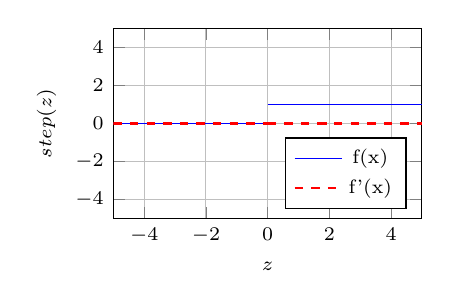
\begin{tikzpicture}
            \begin{axis}
                [width=5.5cm,height=4cm,ylabel=$step(z)$,xlabel=$z$,ymin=-5.0,ymax=5.0,xmin=-5,xmax=5,
                legend style={at={(0.95,0.05)},anchor=south east},]
                \addplot[blue,smooth, domain=-5:0] {0};
                \addplot[red,dashed, thick, domain=-5:0] {0};
                \addplot[blue,smooth, domain=-0:5] {1};
                \addplot[red,dashed, thick, domain=-0:5] {0};
                \addlegendentry{f(x)}
                \addlegendentry{f'(x)}
            \end{axis}
        \end{tikzpicture}
    }
    \subfigure[Linear]{
        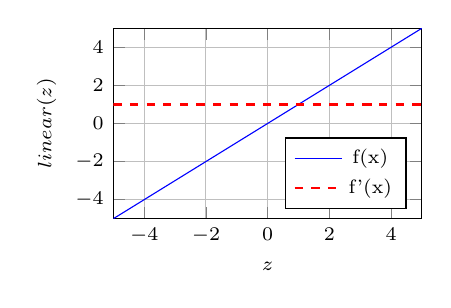
\begin{tikzpicture}
            \begin{axis}
                [width=5.5cm,height=4cm,ylabel=$linear(z)$,xlabel=$z$,ymin=-5.0,ymax=5.0,xmin=-5,xmax=5,
                legend style={at={(0.95,0.05)},anchor=south east},]
                \addplot[blue,smooth] {x};
                \addlegendentry{f(x)}
                \addplot[red,dashed, thick] {1};
                \addlegendentry{f'(x)}
            \end{axis}
        \end{tikzpicture}
    }
    \subfigure[Sigmoid]{
        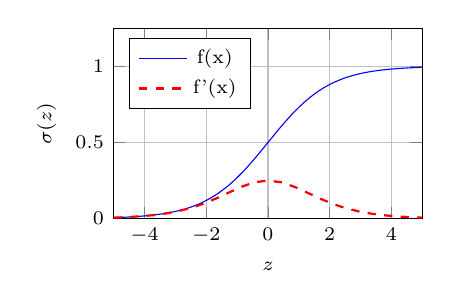
\begin{tikzpicture}
            \begin{axis}
                [width=5.5cm,height=4cm,ylabel=$\sigma(z)$,xlabel=$z$,ymin=0,ymax=1.25,xmin=-5,xmax=5,
                legend style={at={(0.05,0.95)},anchor=north west},]
                \addplot[blue,smooth] {1/(1+exp(-x))};
                \addlegendentry{f(x)}
                \addplot[red, dashed, thick] {1/(1+exp(-x)) * (1-1/(1+exp(-x)))};
                \addlegendentry{f'(x)}
            \end{axis}
        \end{tikzpicture}
    }
    \subfigure[Hyperbolic tangent]{
        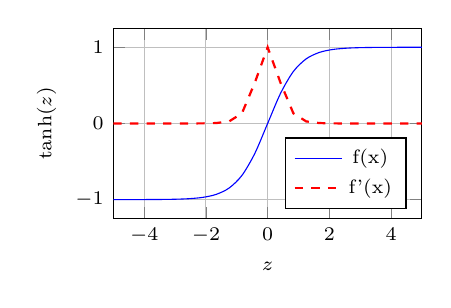
\begin{tikzpicture}
            \begin{axis}
                [width=5.5cm,height=4cm,ylabel=$\tanh(z)$,xlabel=$z$,ymin=-1.25,ymax=1.25,xmin=-5,xmax=5, legend style={at={(0.95,0.05)},anchor=south east},]
                \addplot[blue,smooth] {tanh(x)};
                \addlegendentry{f(x)}
                \addplot[red,dashed, thick] {1/cosh(2*x)*1/cosh(2*x)};
                \addlegendentry{f'(x)}
            \end{axis}
        \end{tikzpicture}
    }
    \subfigure[ReLU]{
        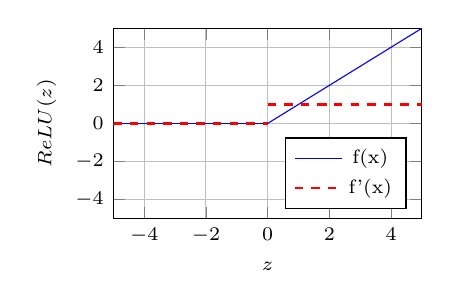
\begin{tikzpicture}
            \begin{axis}
                [width=5.5cm,height=4cm,ylabel=$ReLU(z)$,xlabel=$z$,ymin=-5.0,ymax=5.0,xmin=-5,xmax=5,
                legend style={at={(0.95,0.05)},anchor=south east},]
                \addplot[blue,smooth, domain=-5:0] {0};
                \addplot[red,dashed, thick, domain=-5:0] {0};
                \addplot[blue,smooth, domain=-0:5] {x};
                \addplot[red,dashed, thick, domain=-0:5] {1};
                \addlegendentry{f(x)}
                \addlegendentry{f'(x)}
            \end{axis}
        \end{tikzpicture}
    }
    \subfigure[Leaky ReLU]{
        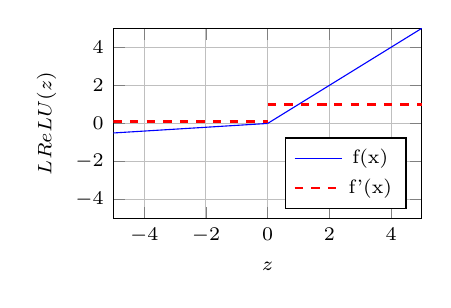
\begin{tikzpicture}
            \begin{axis}
                [width=5.5cm,height=4cm,ylabel=$LReLU(z)$,xlabel=$z$,ymin=-5.0,ymax=5.0,xmin=-5,xmax=5,
                legend style={at={(0.95,0.05)},anchor=south east},]
                \addplot[blue,smooth, domain=-5:0] {0.1*x};
                \addplot[red,dashed, thick, domain=-5:0] {0.1};
                \addplot[blue,smooth, domain=-0:5] {x};
                \addplot[red,dashed, thick, domain=-0:5] {1};
                \addlegendentry{f(x)}
                \addlegendentry{f'(x)}
            \end{axis}
        \end{tikzpicture}
    }
    \subfigure[GELU]{
        \begin{tikzpicture}
            \begin{axis}
                [width=5.5cm,height=4cm,ylabel=$GELU(z)$,xlabel=$z$,ymin=-5.0,ymax=5.0,xmin=-5,xmax=5,
                legend style={at={(0.95,0.05)},anchor=south east},]
                \addplot[blue,smooth] {x * 0.5 * (1 + erf(x /sqrt(2)))};
                \addplot[red,dashed, thick] {0.5 * (1 + erf(x /sqrt(2))) + 1/sqrt(2*pi) * (exp(-x*x/2))};
                \addlegendentry{f(x)}
                \addlegendentry{f'(x)}
            \end{axis}
        \end{tikzpicture}
    }
    \subfigure[Swish]{
        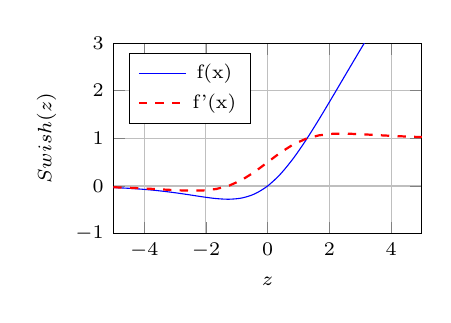
\begin{tikzpicture}
            \begin{axis}
                [width=5.5cm,height=4cm,ylabel=$Swish(z)$,xlabel=$z$,ymin=-1,ymax=3.0,xmin=-5,xmax=5,
                legend style={at={(0.05,0.95)},anchor=north west},]
                \addplot[blue,smooth] {x*(1/(1+exp(-x)))}; % f (x) + σ (x) (1 − f (x))
                \addlegendentry{f(x)}
                \addplot[red, dashed, thick] {x/(1+exp(-x)) + 1/(1+exp(-x)) * (1-x/(1+exp(-x)))};
                \addlegendentry{f'(x)}
            \end{axis}
        \end{tikzpicture}
    }
    \caption[Sigmoidal activation functions.]{Commonly used activation functions in MLPs.}
    \label{fig:activation-functions}
\end{figure}
    \tikzset
{
    myTrapezium/.pic =
        {
        \draw [fill=gray!10] (0,0) -- (0,\b) -- (\a,\c) -- (\a,-\c) -- (0,-\b) -- cycle ;
        \coordinate (-center) at (\a/2,0);
        \coordinate (-out) at (\a,0);
    },
    myArrows/.style=
        {
        line width=0.3mm,
%        red,
        -{Triangle[length=1.2mm,width=3mm]},
        shorten >=2pt,
        shorten <=2pt,
    }
}
\def\a{3}  % width of trapezium
\def\b{1.2} % small height of trapezium
\def\c{2.2}  % tall height of trapezium

\begin{figure}[!htp]
    \label{fig:autoencoder}
    \centering

    \begin{tikzpicture}
    [
        node distance=1mm, % space between drawn parts
        every node/.style={align=center},
    ]


        \node (middleThing)
        [
            draw,
%        fill=purple!80!blue!70,
        %minimum width=1cm,
            minimum height=2*\b cm,
            font=\large,
        ]
        {\begin{tabular}{r}
             $z_1$ \\ $z_2$  \\ $\vdots$ \\ $z_{d_{l}}$
        \end{tabular}};
%    {\begin{tabular}{r}-0.2 \\ -0.1 \\ 0.1 \\ 0.4 \\ -0.3 \\ 1.1\end{tabular}};
        \pic (right)[right=of middleThing.east] {myTrapezium} ;
        \pic (left)[left=of middleThing.west, rotate=180] {myTrapezium} ;
        \node at (right-center) {Decoder} ;
        \node at (left-center) {Encoder};
        \node at (right-center) {Decoder} ;

        \def\d{.9}
        \coordinate (u) at (\d,0);
        \draw [myArrows] (right-out) -- ++(u) node [anchor=west] {$\mathbf{y}$};
        \draw [myArrows] ($(left-out)-(u)$) node [anchor=east] {$\mathbf{x}$} -- ++(u) ;

    \end{tikzpicture}
    \caption{Autoencoder architecture.}
\end{figure}
    \tikzset{basic/.style={draw,text width=1em,text badly centered}}
\tikzset{component/.style={rectangle, draw=black, thick, text width=7em,align=center, rounded corners, minimum height=2em}}

\begin{figure}[!htp]
    \label{fig:agent-environment}
    \centering
    \tikzstyle{block} = [rectangle, draw,
    text width=8em, text centered, rounded corners, minimum height=4em]

    \tikzstyle{line} = [draw, -latex]

    \begin{tikzpicture}[node distance = 6em, auto, thick]
        \node [block] (Agent) {Agent};
        \node [block, below=5em of Agent] (Environment) {Environment};
        \node [left=3em of Environment] (Dashed) {};
        \node [above=1.7em of Dashed] (Dashed-up) {};
        \node [below=1.7em of Dashed] (Dashed-down) {};

        \path [line] (Agent.0) --++ (4em,0em) |- node [near start]{Action, $a_t$} (Environment.0);

        \path [line] (Environment.190) -- (Environment.190-|Dashed-down.east) node [midway, label={[xshift=-0.0em]center:$s_{t+1}$}] {\phantom{$s_{t+1}$}};
        \path [line] (Environment.170) -- (Environment.170-|Dashed-up.east) node [midway, above, label={[xshift=-0.0em]center:$r_{t+1}$}] {\phantom{$r_{t+1}$}};

        \path [line] (Environment.190|-Environment.190) --++ (-6em,0em) |- node [near start] {} node [near start, label={[xshift=-0.0em]center:State, $s_t$}] {\phantom{State, $s_t$}} (Agent.170);
        \path [line] (Environment.170|-Environment.170) --++ (-4.25em,0em) |- node [near start, right] {} node [near start, right, label={[xshift=-0.0em]center:Reward, $r_t$}] {\phantom{Reward, $r_t$}} (Agent.190);

        \draw[dotted] (Dashed-up.east) -- (Dashed-down.east);


    \end{tikzpicture}
    \caption{Agent-environment interaction interface.}
\end{figure}
\end{document}
